\chapter{Tangram: Simplify PCB Design Process with Modularization}

In previous chapter, we started from medical-background users' viewpoints to design a wearable platform for developing health applications.
However, a team to develop an application may involve cross-disciplinary members.
The users with different background knowledge and skill levels have various requirements for prototyping.
Thus, we extend the concept of BioScope and further consider the needs of engineering-background users who develop and implement the device for wearable, mobile and IoT applicxqations.
This process often requires numerous design iterations before reaching its design goals.
In the past, makers have to spent significant efforts on implementing outer cases, electronic components, firmwares and corresponding softwares, while designing and exploring various novel applications.
With the evolutions of technology on 3D printing, laser cutting and CNC engraving, it becomes much easier and affordable for HCI researchers and the emerging makers \cite{maker_fair} to do rapid prototyping on the appearance of devices. 
%However, makers still spend a lot of effort and time on prototyping electronic part of devices on each design iteration.

For developers to prototype on digital functionalities, Arduino, by providing easy-to-use hardware and software, is the most popular open-source development toolkit.
However, users may meet some problems with using such development tools to prototype their devices.
Robustness would be an important issue when users will have tangible interactions with the device.
Troubleshooting of a bunch of wires bridging the main controller and external components will bring a lot of bother to users.
Also, a device built by development tools may not be able to meet users' needs in dimensions and power saving
To address these issues, many HCI researchers then choose to build their device with customized PCB, which has high quality with low cost \cite{seeed_fusion, smart_prototyping}. Nevertheless, designing PCB is not only a hard work for those who has no background knowledge, but it also costs experienced users a lot of time and effort.

In HCI community, several attempts have been made on reducing the effort spends on prototyping and fabrication processes.
D.tools \cite{dtool:2006} proposed a toolkit that supports design thinking processes for device prototyping with iteration cycle between analysis, designs and testings. 
Knibbe et al. \cite{Makerspace:2015} built the Smart Makerspace to guide makers to build devices with immensely instructed environment. %% what part of device?
FaBrickation \cite{Mueller:2014:FFP:2556288.2557005} presents an approach on speeding up 3D printing process by substituting sub-volumes of devices with standard building blocks. %% this is the appearance part
Previous researches \cite{Printem:2015, inkjet_circuits:2013} demonstrate how to fabricate PCB for rapid prototyping using a standard inject printer. %% electronic parts?
%% problem: not quite sure about the purpose of this paragraph and the relationship between the text.

This work introduces a system designed for makers to build a customized PCB effectively avoiding tedious tasks.
The system consists of two parts: (1) TangramScope, a flexible and extensible physical developing toolkit; and (2) TangramFab, a modular PCB layout software.
TangramScope allows developers to select required components for prototyping and evaluating the functions of a dedicated device for their application. 
After the functionalities of devices built by TangramScope reach expectation, developers can easily import the configurations into TangramFab.
With a few more customization settings, TangramFab can generates all necessary design files for PCB fabrication.

\section{Design considerations}

Developers usually go through several design iterations before their products reaches their design goals using off-the-shelf developing toolkit (e.g., Arduino or Raspberry Pi) and peripheral components (e.g., sensor modules, actuators, displays, etc.) in early stages.
To better understand the needs in making electronic devices, we conduct semi-structure interviews on 6 participants, who have experience on HCI projects (4 male and 2 female age from 22 to 33 with computer science or electrical engineering background).
We also demonstrated our early prototype with a simple example, a device equips Bluetooth radio and 9-axis motion sensor, to collect their feedbacks and comments.
In this section, with lessons learned from our study and observations, we describe the challenges to develop a system that assist rapid prototyping with high quality customized devices.

%%Delete this sentence "Prototyping with development toolkits is simple task to all of our participants, because adequate online resources including tutorial and software library can be easily find." Not sure what does this sentence wants to show.



\subsection{Prototyping with off-the-shelf developing toolkit}
We summarize several issues below, reported by our participants based as their experience to prototype with off-the-shelf developing toolkit.

\subsubsection{Robustness}
Robustness is the most-frequently reported reason that drives developers to fabricate customized PCB board.
Developers complained that off-the-shelf developing toolkit often have issues on poor connections and wires being pulled out while testing, especially when they use jumper wires or cable connectors for devices in mobiles, wearables, and interactive applications.
Developers also mentioned that it costs a lot of time on connecting the wires correctly.

\subsubsection{Form factor}
Most of the off-the-shelf developing toolkits are designed to support general purpose and extendibility, equipped with more components and interfaces to communicate with different external components.
The result is that they usually have larger size and heavier weights.
In many cases, developers then have to fabricate customized PCB boards with ideal shape and compact size for their applications.

\subsubsection{Power consumption}
One of our interviewee reported that a device's battery life is a key effect on a long-term user study. 
Short battery life causes bad user experience, enabling power saving mechanism is important to prolong the battery life.
However, off-the-shelf developing toolkits may not be able to support power saving due to the hardware configurations.



\subsection{Fabricate customized PCB}
To address the above issues caused by using off-the-shelf developing toolkit, developers therefore have to customize PCB to build high-quality electronic devices.
However, developers still confront several challenges when designing PCB.

\subsubsection{Difficulties in implementations}
All of our participants agree that PCB design requires relatively high technical skill and background knowledge, comparing to off-the-shelf developing toolkit.
Challenges accounted in different stages of design process are:
(1) Besides simply select components that matches their requirements, developers have to spend a lot of time on checking the compatibilities between each components.
(2) Different setting on components produce difference functionalities on the same component, e.g., power saving mechanism relies on secondary oscillator and correct power regulation in hardware.
Developers may misconfigure their components if they do not have enough information.
(3) Correctness of the circuit board is another difficulty, since developers may only notice the errors after the board is fabricated.
The entire PCB will not work even there is only a mistake in a single pin or wire.
Although there are many PCB design softwares that check design and electrical rules automatically, logical errors are still inevitable.
(4) A beginner may get stuck to getting started in PCB design, if he/her doesn't have relevant background knowledge.
%Spend a lot of time reading documents to put on the right capacitors, resistors, etc.?
%% (5) Rewriting the software code after changing from Arduino to PCB?

\subsubsection{Cost}
Nowadays, although the price of PCB fabrication service has decreased significantly, the overall cost on time, money and effort is still considerably high for developers.
To prevent revisions caused by unexpected behaviors and misconfigurations, it is important to provide physical testing on their PCB designs and generate correct PCB designs afterwards. %% mapping to TangramScope and TangramFab


%% Delete "Some developers therefore prefer to build their devices with off-the-shelf developing toolkit when the quality is acceptable." (Not sure why this sentence is here)


\begin{figure}[ht]
\begin{center}
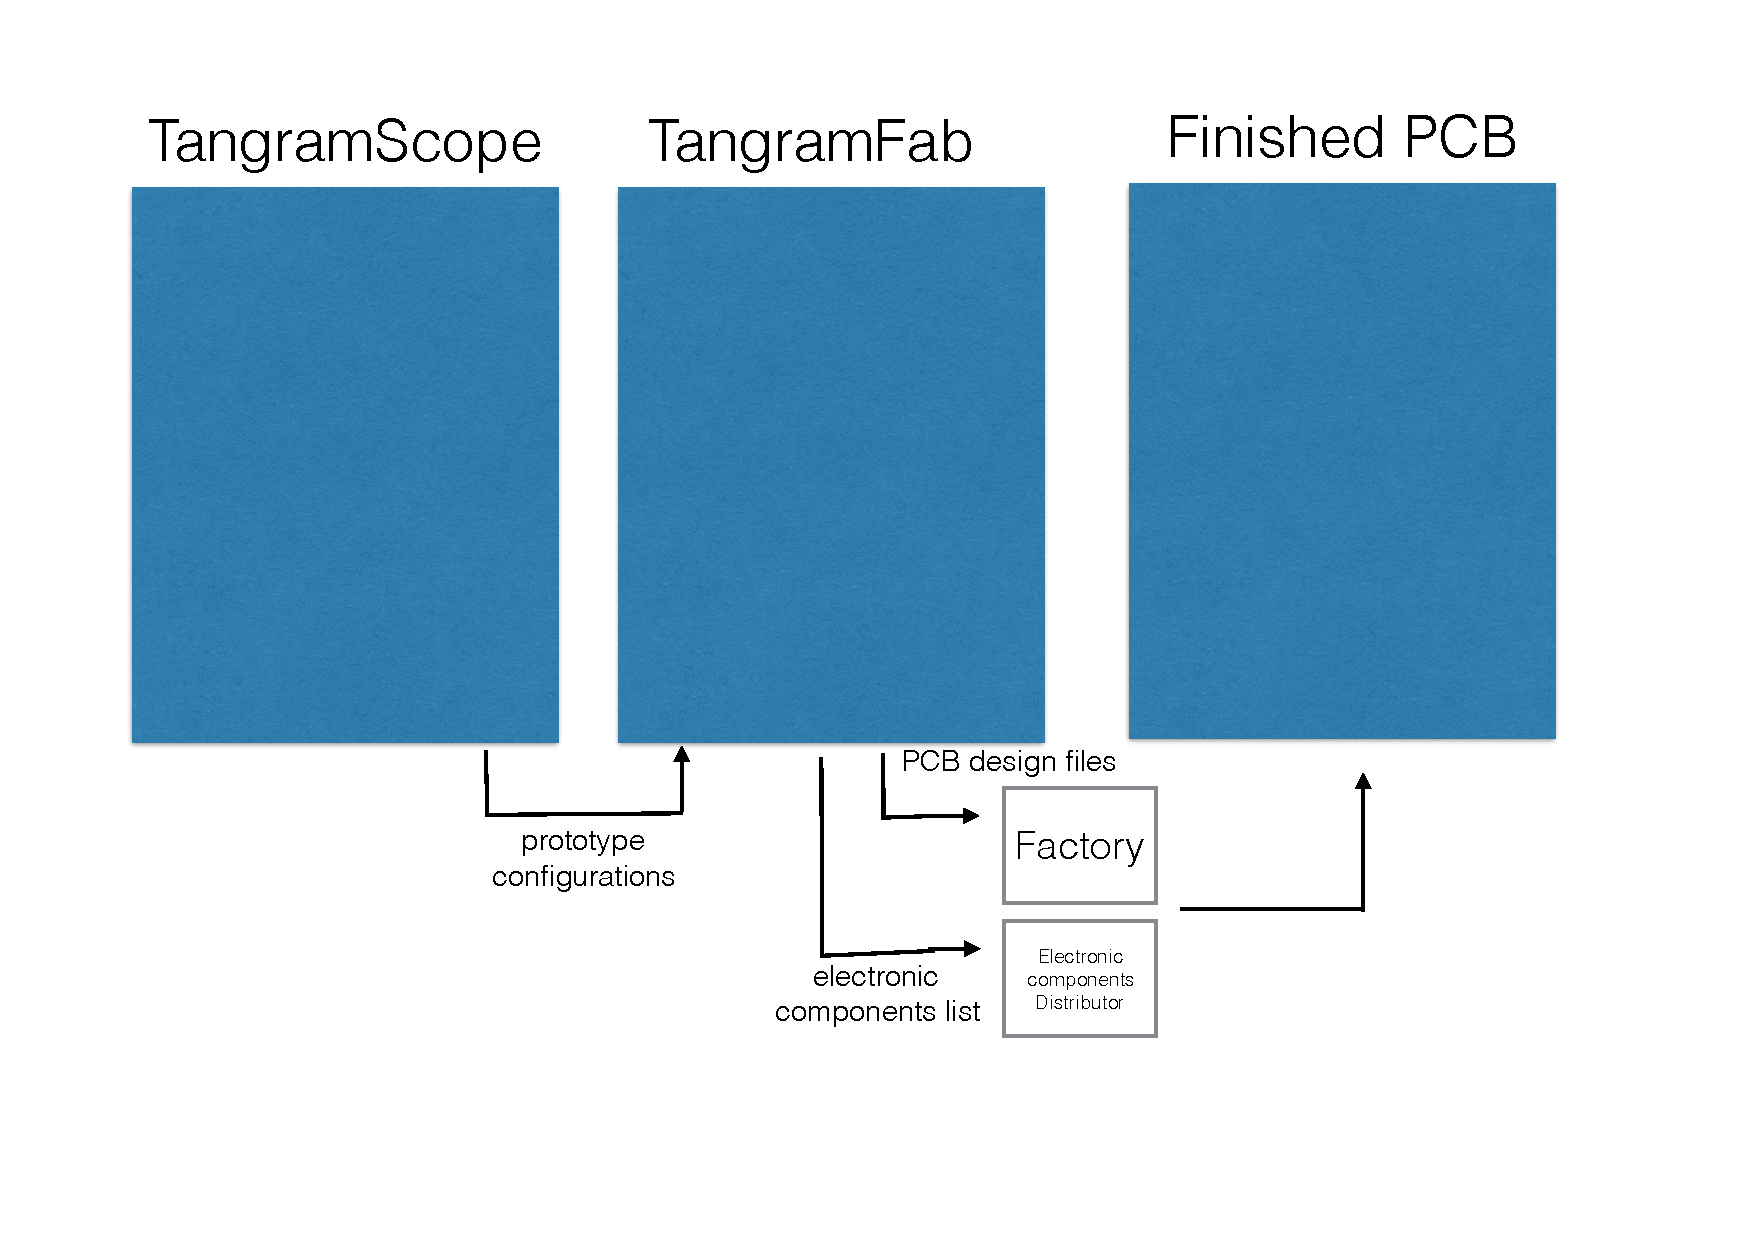
\includegraphics[height=10cm]{image/tan/flowchart.pdf}
\caption{Flowchart of the Tangram.}
\label{fig:flowchart}
\end{center}
\end{figure}

\section{System design}
%To simplify the procedure on creating a customized PCB, we propose the system with two parts: (1) TangramScope, a flexible and extensible development toolkit; and (2) TangramFab, a modular PCB layout software.
%Figure ? shows the entire flow using our service. 
%Developers can firstly prototype the device using TangramScope for evaluating and testing the device whether can conform with their applications.
%Then the configuration of the prototype (e.g., the components used, parameters of the components, connections between components) will be automatically imported into TangramFab for further PCB design.
%With TangramFab, developers can easily design the shapes of their boards and arrange the locations of the components according to their needs.
%After developers have completed the layout of the circuit board, TangramFab exports the shopping list of the components used on the board and the design files with standard format required by the factory for PCB fabrication.

To simplify the procedure of creating a customized PCB, we propose a service with two parts:
(1) TangramScope, a flexible and extensible physical development toolkit;
and
(2) TangramFab, a web-based PCB layout software with modular components.
A Tan is a module that wrap the main electronics components, (e.g., chips),capacitors, oscillators, etc.

Figure~\ref{fig:flowchart} shows the entire flow of our service.
Developers can first easily prototype their devices using TangramScope to evaluate and test their prototypes.
After their prototypes conform to their applications, the configurations of their prototypes (e.g., the components used, parameters of the components, connections between components) will be automatically imported to TangramFab.
Developers use TangramFab to design the shapes of their boards and arrange the locations of the components according to their needs.
TangramFab then exports the standard design files required for PCB fabrication.
Finally, by sending the standard design files and electronic components to PCB Manufacturer, the final PCB is made.

With our system, developers avoid issues when using off-the-shelf development toolkit and difficulties when customizing PCB board in the ordinary way.
First, with customized PCB, the device is more robust and can be made into desired shapes.
Second, all Tans in our system have no compatibilities problem between Tans and are designed with power saving mechanism.
Third, each Tan has only one function. Electronic components that have different function according to their configurations are separated into different Tans with corresponding configurations.
Fourth, since the Tans in TangramScope and the Tans in TangramFab differ only from the position of electronics components within and connectors between Tans, the final PCB works exactly like the prototype built with TangramScope. In addition, programs that runs on TangramScope can also run on the final PCB without modification.

\begin{figure}[ht]
\begin{center}

\includegraphics[height=8cm]{image/tan/space.png}
\caption{(a) Tans of TangramScope. (b) Stacking mechanism.}
\label{fig:TangramScope}
\end{center}
\end{figure}

\subsection{TangramScope}
Since there is no chance to turn around after standard format files are sent to factory, most developers prototype their devices with an off-the-shelf development toolkit before designing a dedicated PCB.
In this work, we present TangramScope, a flexible and extensible development toolkit that allows developers to easily prototype their electronic device and evaluate their design.
We leverage the same design concept as well as BioScope, and extend the application area to mobile and IoT.
In addition, the previous code running on TangramScope can also run on the PCB produced by TangramFab without modifications.
By programing the prototyped device with the peripheral detection firmware , the configuration of selected Tans can be captured and then output to TangramFab for further PCB layout process.

To demonstrate the design of TangramScope, we implement several sample modules (Figure \ref{fig:TangramScope}(a)) including microcontroller board, Bluetooth radio board, motion sensor, temperature sensor, ECG heart rate sensor, camera, OLED display, microphone, audio DAC, flash storage, RFID reader and Lithium-battery recharger.
TangramScope provides the hands-on platform for prototyping that can assist developer to design a customized PCB with correctness in TangramFab.
TangramScope adopts the stacking mechanism that developers can easily assemble modular components through compact 30-pin connectors like LEGO bricks.
The connectors involve SPI and I2C bus that the modules can communicate to each others, and provides battery power and regulated 3V supply voltage sourced from microcontroller board (Figure \ref{fig:TangramScope}(b)).


\subsection{TangramFab}
TangramFab is a web-based UI that let users arrange the desired Tans to form shapes that matches their applications.
Developers can either use information imported by TangramScope or start from scratch with TangramFab.
TangramFab is divided into three main parts: the Workspace, the Tan library and the TodoList, as shown in Figure~\ref{fig:tangramFab-comment}.
The Workspace is where developers situate Tans and draw the dimension of the final PCB board.
Tans that are not on the workspace can be added by dragging items from the Tan library below.
Key information (e.g., number of pins, bus type, etc.) of the Tans are displayed for developers.
The TodoList on the right helps developers get track of missing Tans and warnings from system.
After editing, TangramFab will output a BOM (bill of material) file of used components and standard design files for fabrication including Gerber, stencil and pick $\&$ place files.
The BOM file can be imported to the shopping cart of online electronic components distributor (e.g., Mouser, Digikey, etc) for purchasing required electronic components..


\begin{figure}[!h]
\begin{minipage}[t]{1\columnwidth}
  \centering
  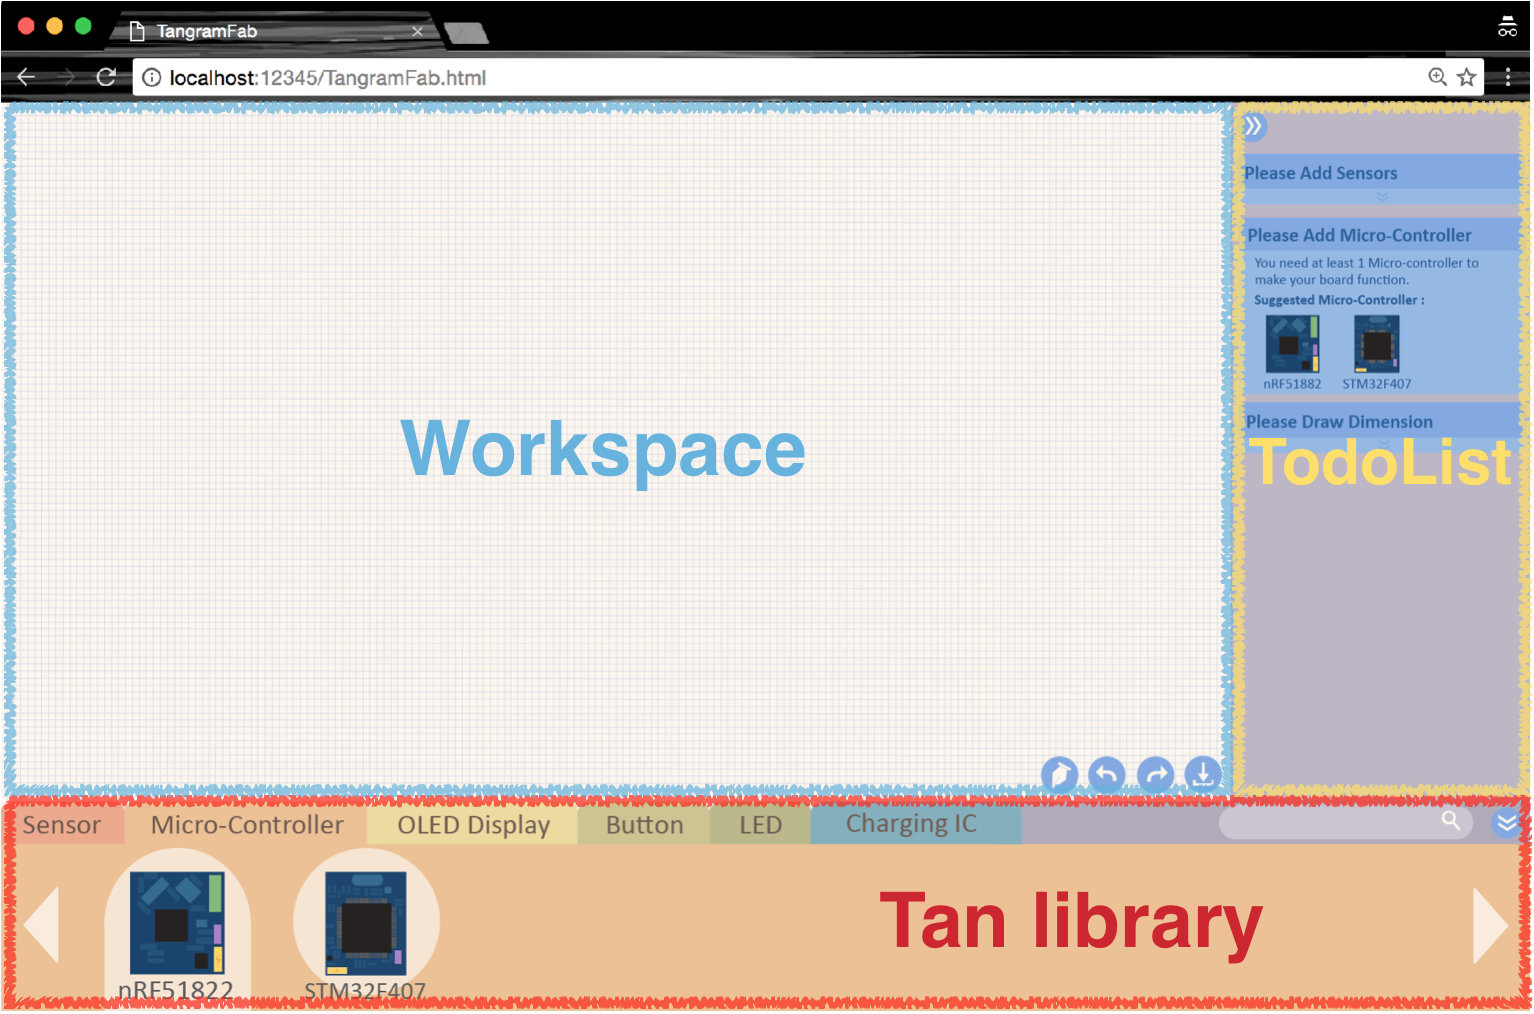
\includegraphics[width=1\textwidth]{image/tan/TangramFab-Comment}
  \caption{Snapshot of TangramFab.}\label{fig:tangramFab-comment}
\end{minipage} 
\begin{minipage}[t]{0.47\columnwidth}
    \centering
    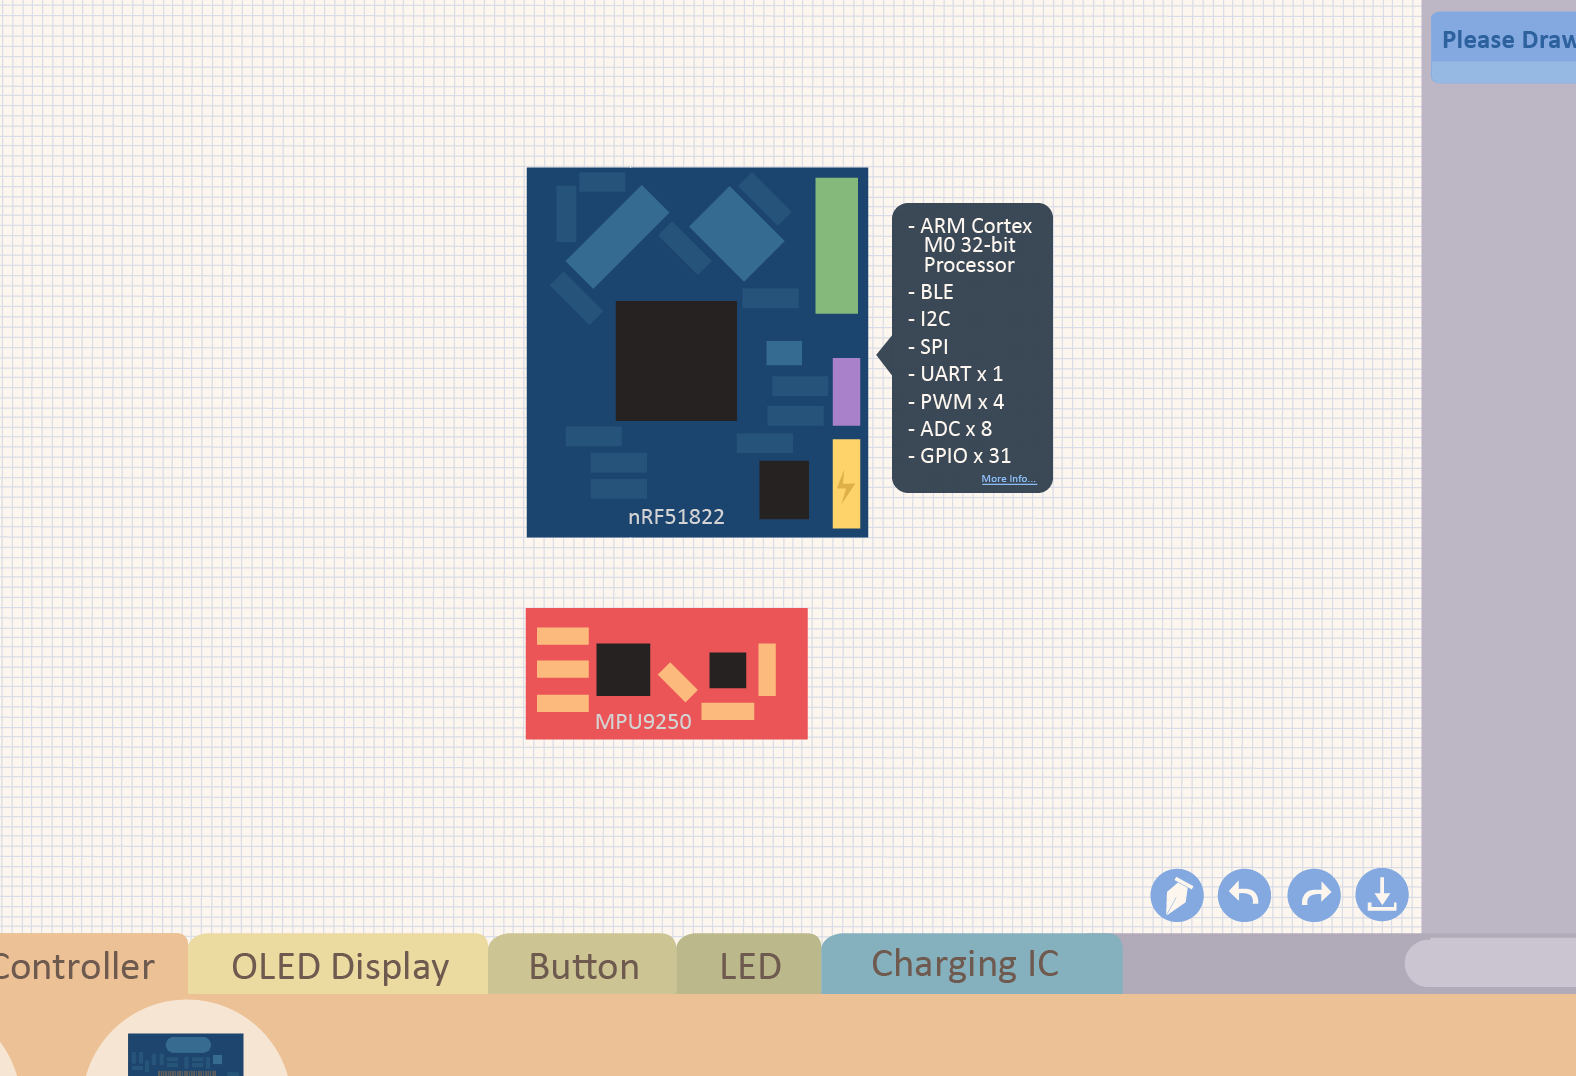
\includegraphics[width=1\textwidth]{image/tan/TangramFab-Initial}
    \caption{Tans imported into TangramFab from TangramScope.}\label{fig:tangramFab-initial}
\end{minipage}
\hspace{0.1cm}
\begin{minipage}[t]{0.47\columnwidth} 
    \centering
    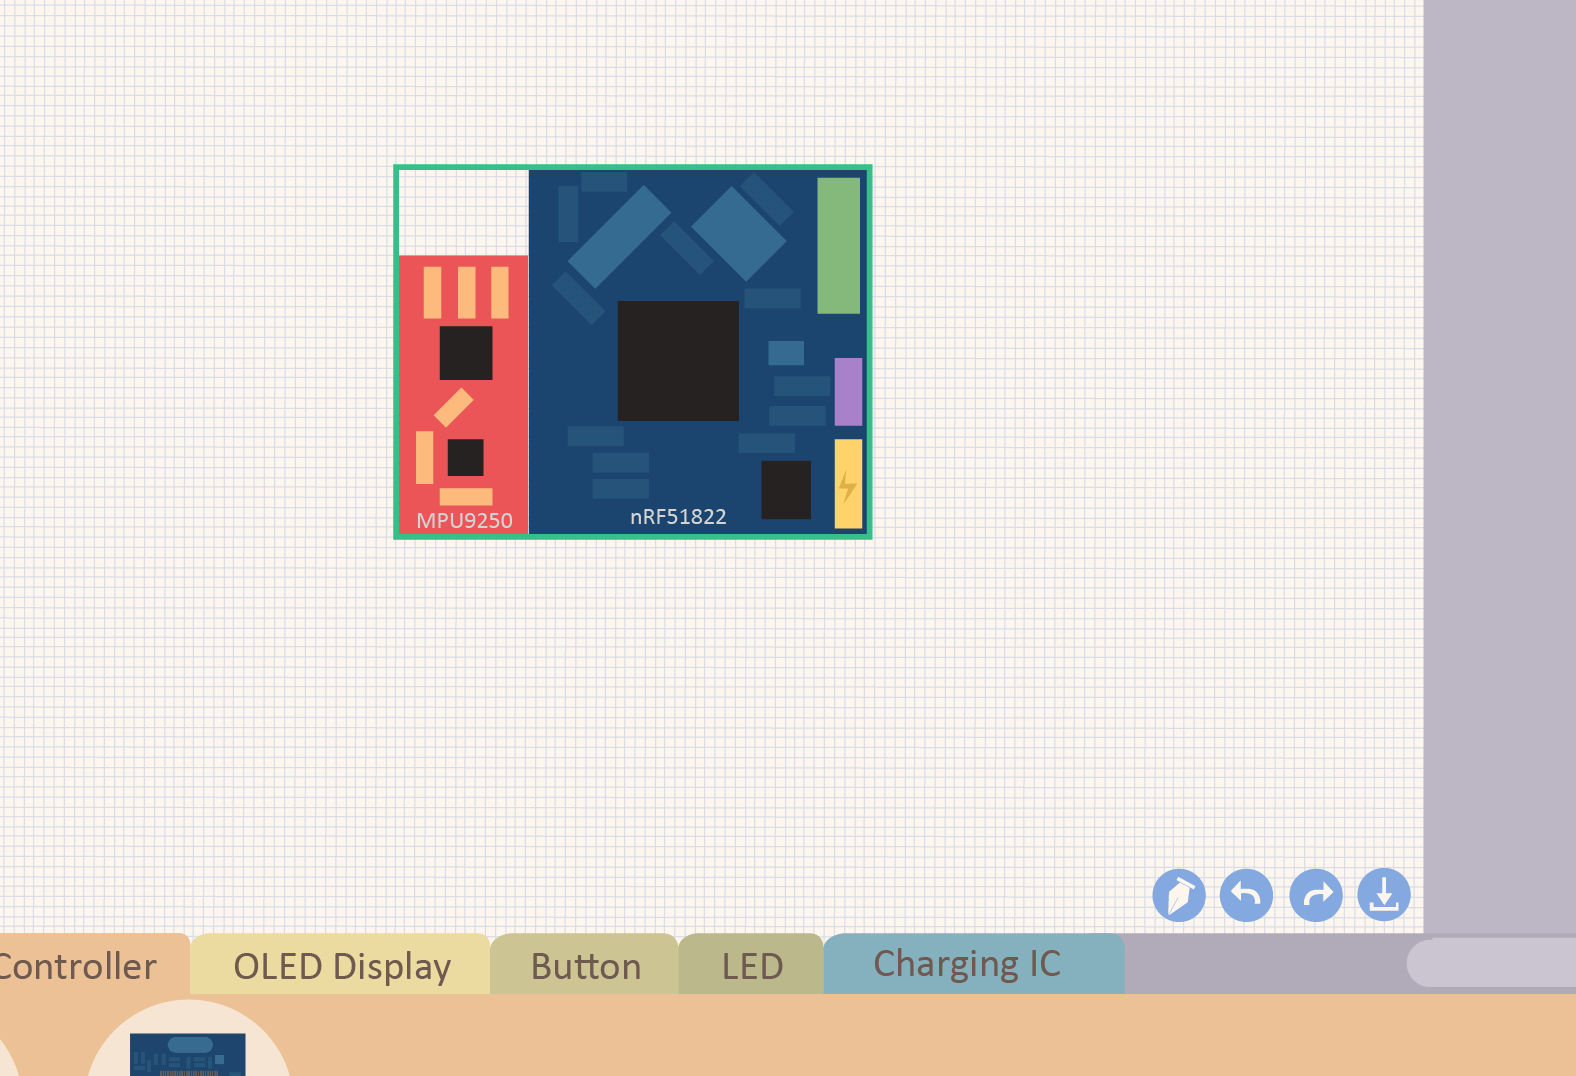
\includegraphics[width=1\textwidth]{image/tan/TangramFab-Final}
    \caption{Situate Tans to desired positions and draw the dimension.}\label{fig:tangramFab-final}
\end{minipage}        
\end{figure}  

\subsubsection{Sample scenario}
Here we have an example to show how developers use TangramFab to produce PCB designs.
To build a device with a bluetooth radio (Nordic nRF51822) and a 9-axis motion sensor (InvenSense MPU9250), developers first use TangramScope to build their prototype and test it with their programs.
With TangramScope the settings are then imported into TangramFab as Figure~\ref{fig:tangramFab-initial}.
Developers can alter the default configurations of a Tan (e.g., type of connector, battery, etc) if needed.
Developers then rotate and move the Tans, which is the motion sensor here, according to their needs.
After developers draw the dimension of the PCB board as Figure~\ref{fig:tangramFab-final} and click the export button, the components list and standard files for fabrications are produced.

\begin{figure}[tb]
  \centering
  
\includegraphics[width=1\columnwidth]{image/tan/space1.png}
  \caption{(a) The toy doll embedded electronic device. (b) The customized PCB.}\label{fig:study}
\end{figure}

\section{Explorative study}
We recruited one participant from previous interviews to explore and evaluate the capability of our design.
The participant seeks PCB customization for his project, but doesn't have experience in PCB design.
The goal is to build a toy doll \cite{Wakey:2017} embedded electronic device (Figure \ref{fig:study}(a)) that can interact with children to guild children's daily routine without procrastination, e.g., get up and breakfast.
He first prototyped his device using Raspberry Pi, sensor modules, microphone and  speaker.
In previous interview, he reflected that he is discontented with and robustness, size, weight, battery life and cost of the prototype built by these components.
He therefore want to customized the device for addressing these issues.

Based on the interview with the participant, we prepared the TangramScope modules with sample codes according to the requirement of his device, including the microcontroller board, camera module, microphone, audio DAC and RFID reader.
After the hands-on prototyping with TangramScope, the configuration is exported to TangramFab for PCB design.
With several steps to layout on TangramFab, the system generated PCB design files and sent to factory for fabrication (Figure \ref{fig:study}(b)).

When the customized PCB has arrived, we conducted a interview the participant to collect feedback.
The participant commented: \textit{``As a beginner in PCB design, I feel it is hard to getting started to know how to do part selection. That would be nice to have some examples to see what components they typically used in their applications. $\cdots$  When I make my circuit board with TangramFab, I had some doubts that can really produce what I want with those simples steps. Although I have yet program my codes on this board, all modules on the board function correctly as I expected with demo codes. I think it will work well in my application. And the finished PCB is much compact and light weight than my previous prototype!}''
As the result, our system can assist participant to produce a customized PCB that can really meet the requirements for his application.

%For another example, a participant prototyped his device using Raspberry Pi supplied by a USB power bank.
%He stated that his device runs out of battery so fast even his adapted a heavy power bank.
%Therefore, he would like to find a low power solution for his application.


\section{Discussion}

\subsection{Flexibility and Difficulty in PCB Design}
Conventional PCB design software provide the flexibility to design any details on the board.
Considering the threshold is high for the beginning developers who do not have required skills and background knowledge in PCB design.
We design our system with modularization that can simplify the PCB design process by finding a balance between flexibility and difficulty.
With our system, developers can build a customized PCB without undergoing low-level design processes.

\subsection{Developing a Well-provisioned Library}
As a proof-of-concept system, we provide only limited Tans in current TangramScope and TangramFab.
A well-provisioned library is a necessary condition to provide good usability of this system for users.
The crowd's power would be a possibility to achieve this goal.
For example, Arduino has a great community that have contributed a comprehensive library and tutorials that people can easy to access.

\subsection{Limitation and Future Work}
In this work, we studied a small group of participants our system still has room to improve the usability and the limited library.
Many participants in our study reflected the importance of supporting users in software programing with our system.
Many developers may already familiar with a development tool.
TangramFab should be compatible with other development toolkits by designing a system that can transfer the configurations of prototype device for PCB design.
For advanced developers who may desire more flexibility to customize their PCB, they can  also get benefits in our system.
We will provide the function that can export the layout in TangramFab to external PCB design software (e.g., Eagle format in XML \cite{eagle}) that developers can further edit the details of the layout.
Thus, our system can assist they to rapidly generate a reference design that contain all required electronic component to save the time.

\section{Summary}
In this work, we intend to refine the conventional process of building an electronic device by considering and exploring the balance between flexibility and difficulty.
TangramScope, a flexible and extensible development toolkit, allows users to build an electronic device by choosing modular components for prototyping their application.
Developers can evaluate and test the device built by TangramScope whether the functions are working properly as they expected.
TangramFab, a modular PCB layout software, provides a UI for simplifying PCB layout process.
Our explorative study demonstrates how this system can assist users to rapidly prototype their design and easily build the customized PCB.
